\chapter{Implementation}

\section{Technologies}
With a clear picture of the requirements and the aspired architecture, it is time to talk about technology, which programming languages will be used and what are the main libraries.

\subsection{Frontend}
One of the requirements is for Sparked to be a web application. Therefore the frontend will ultimately be in HTML, JavaScript, and CSS, the web stack. With Flash and Silverlight support finally ending in 2020 and 2021 respectively \cite{silverlight} \cite{flash} there really is no alternative. There are however several ways how to get to this HTML, javascript, and CSS.

\subsubsection{SPA}
There are numerous ways to create dynamic websites. One of them is the use of a Single Page Application (SPA) framework. SPAs work in such a way that the main page is only loaded and the Document Object Model (DOM) only evaluated once by the browser. Then JavaScript is used to make server calls, animate objects, bind event handler to actions, change the DOM and do everything else that is required for the website to function. This means that the UI is effectively been built in the browser on the client machine.

\subsubsection{Angular}
For this project, the choice of SPA framework fell on Angular. This is not for any specific technological reason, as all the well-known SPA frameworks can support anything needed by this project, instead, the choice was made because of previous know-how existed. 

Angular is maintained by Google, was first released in 2009 \cite{angularJS} and is available under a modified MIT license \cite{angular}, with the newest Version being 8.0.0, released on May 28th, 2019 \cite{angularRelease}. Sparked uses Version 7.2.3 as it was the newest at development time. 

Angular uses TypeScript as a programming language. TypeScript is a superset of JavaScript extending it with features like inheritance and strongly typed variables. It being a superset means that all valid JavaScript code is also valid in TypeScript. That is not true the other way. Instead, TypeScript uses a preprocessor to compile TypeScript code into JavaScript before deploying it to the client. 

TypeScript is an open source project available under the Apache License 2.0 \cite{typescriptLicense} and was first released by Microsoft in 2012 and exists now in Version 3.4 \cite{typescript}. Sparked uses the Version 3.2.4. 

\subsubsection{Node Package Manager}
When working with angular it is recommended to use the NodeJS and the node package manager (npm) to install and manage angular and the libraries used by angular.

\subsubsection{ChartJS}
As seen in the previous chapter, Sparked needs a way to display data as graphs. There are a lot of charting frameworks available. From commercial libraries such as Highcharts, over free software like google charts to free open source projects like Chartist. There are some characteristics for a charting framework to be considered in this project. The library should be free to use without constraints like watermarks. A couple of chart types must be included and while scatter-, line- or box charts are rather standard, box and whiskers plots are only supported in some libraries. 

For this project, the decision fell on ChartJS. It is available under the MIT license \cite{chartjs}, can be used with the node package manager and has an active community behind it \cite{chartjs-contributors}. It supports all standard plot types and with the help of an extension, chartjs-chart-box-and-violin-plot, it supports box and whiskers plots. The version used is 2.8.0.

\subsection{Backend}
Having looked at the client-side technologies it is now time to do the same for the server side. 
\subsubsection{Java}
Almost every major programming language today has libraries, that allows creating a simple CRUD web server. As such the question which language to use is not so much dependent on the features of the language itself but more on the level of knowledge current and future developers might have in it. With this Java becomes a safe bet as it is one of the most widely used programming languages \cite{stackoverflowSurvey}. 

When it comes to creating web application backends with java Spring Boot, here used in version 2.1.1 is a widely used and powerful tool that will reduce the configuration overhead and supplies powerful tools to the development project. 

\subsubsection{Database}
For data storage MongoDB, a document based No-SQL database was chosen. MongoDB is a tried technology with existing drivers for Java. The main benefit of a schema-less database like MongoDB is, that changes in the data do not need to be consciously reflected in the database. This makes changes to Sparked easier, as it reduces the points in code that need to be changed if the CODA API were to change. For the database driver, MongoDB-driver in version 3.8.2 was chosen.
\subsubsection{Serialization}
The Sparked backend gets data from the Coda API on one side and sends data to the UI on the other. Both are sent in JavaScript Object Notation or JSON format. To convert said data from JSON to what is often called a POJO, a plain old java object, to work with it on the Server and back to JSON, a serialization function is needed. Using Jackson this process can be automated converting JSON objects to Java objects without the need to write converters. Jackson will instead try to convert them automatically using reflection and a combination of conventions and attributes to map JSON to Java values. This has the added benefit, that a change in the underlying API in many cases only needs for the transformed object to be adapted. In comparison, the change of a handwritten serializer or deserializer would take up much more time. 
\subsubsection{Swagger}
The Sparked backend publishes an API for consumption by the angular frontend. While this is an internal API and does not technically need to be documented, it will be helpful for future developers to see all valid endpoints and their usage in one spot. Swagger is the tool of choice when it comes to API documentation. It creates a page at the relative path \textit{\/swagger-ui.html\#/} that shows an overview of all endpoints and shows supported parameters, responses that can be expected and the data structures of return values. This information should enable frontend developers to change the UI or even create a new one without having to go into the code themselves. 

\begin{figure}
	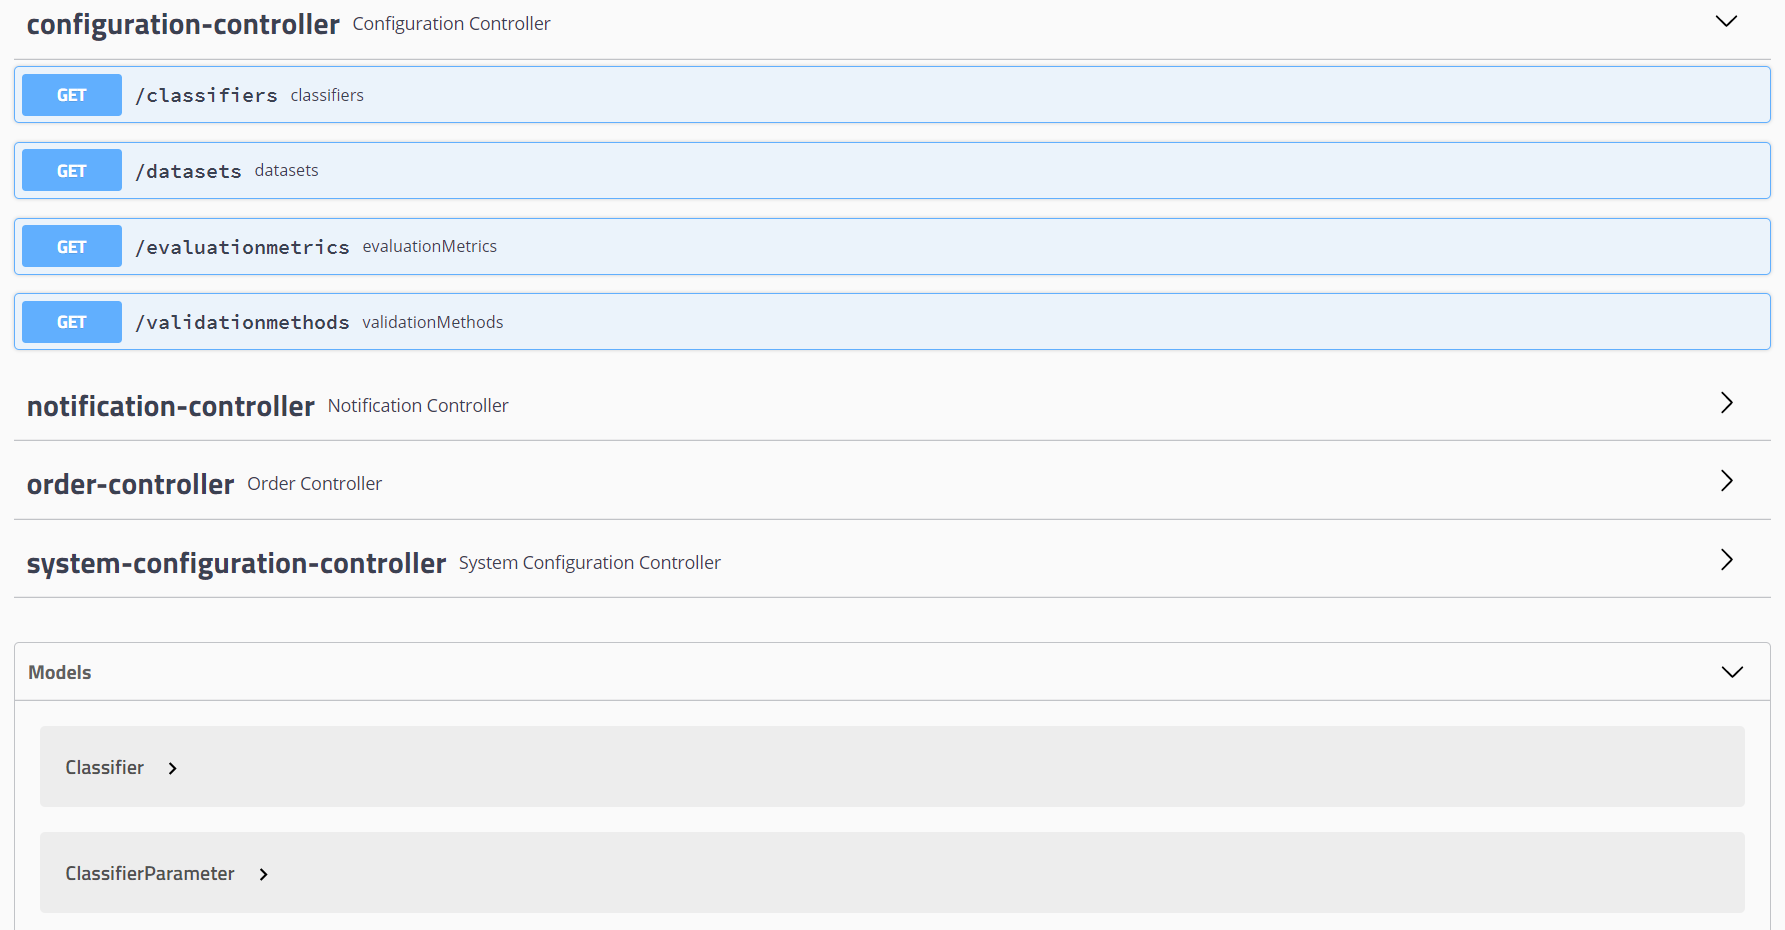
\includegraphics[width=\textwidth]{Swagger.png}
	\caption{The Swagger UI shows a synopsis of Sparkeds web-API}
\end{figure}


\section{Noteable code}
\subsection{Coda API}
The ML functionality of Sparked comes fully from CODA via the CODA API \ref{appendix:CodaAPI}. The CODA API returns JSON Objects, which is where Jackson comes into play. Jackson maps objects from JSON to the corresponding Java object. It makes the connection either by property name or by using attributes.

\begin{lstlisting}[caption={Metric returned by the CODA API in Json format.},captionpos=b]
{
	"id": "class specific specificity",
	"highValueBetter": true,
	"isScalarMetric": false,
	"isClassSpecific": true
},
\end{lstlisting}

\begin{lstlisting}[caption={Metric class in Sparked. The fields match the Json fields.},captionpos=b]
@JsonIgnoreProperties(ignoreUnknown = true)
@JsonInclude(JsonInclude.Include.NON_NULL)
public class Metric {
    private String id;
    private Boolean highValueBetter;
    private Boolean isScalarMetric;
    private Boolean isClassSpecific;
\end{lstlisting}

This is a fast and reliable way to serialize and deserialize the data. Since it maps by using known names, this method only works with known named properties. For properties where the property name is not constant, this does not work. CODA, for example, puts an id before the classifier parameters. For this Jackson supports custom deserializer. 

\begin{lstlisting}[caption={Objects with changing variable names need a more complex deserialization procedure.},captionpos=b]
"results": {
"bestConfiguration": {
     		"params": {
              "dtc_6b195ee4e3bb__seed": "159147643",
              "dtc_6b195ee4e3bb__cacheNodeIds": "false",
              "dtc_6b195ee4e3bb__checkpointInterval": "10",
              "dtc_6b195ee4e3bb__impurity": "gini",
\end{lstlisting}

Having a component do what otherwise would be many hundred lines of custom code is already worth adding a library, but the main benefit here becomes apparent when trying to expand the CODA data structures. Because the database is schema-less and the frontend is compiled into JavaScript, neither of these parts need to be changed to support additional fields in CODAs data structures. The only change needed is to create matching variables as well as getter and setter functions in the corresponding Java class and the values should become accessible in the frontend.

Of course, this only works on auto mapped classes. If the evaluation result data were changed, both the matching class as well as the deserializer, EvaluationResultMetricDeserializer, would need to be edited. Changing the deserializer is not the biggest issue, but it is to be noted, that for an earlier version of CODA API several deserializer classes existed with one having more than a hundred line of low-level code to traverse and read Json nodes. Changing a class like that can quickly become hard and is an easy place to make errors. 

\subsection{Configuration}
The configurable data in Sparked concerns three issues. The first issue is the MongoDB connection, containing IP-address, port, database name, and collection name as well as timeout values. Another property in this block is the clear\_database\_on\_startup property. If set to true, it will drop the MongoDB collection, deleting all saved Orders. This effectively clears all existing Orders from the program on startup.

The second is the CODA connection, containing the APIs IP-address and port value as well as the polling interval in which to query the backend for changed status information as described in the Order list workflow description.

\begin{lstlisting}[caption={The config.properties file.},captionpos=b]
mongo_Port=8080
mongo_IP=40.68.62.58
mongo_Database_Name=coda_db
mongo_Collection_Name=orders
mongo_Connection_Timeout=1000
mongo_Server_Selection_Timeout=0
mongo_Socket_Timeout=1000
clear_database_on_startup=false

order_Status_Intervall=60
coda_backend_ip=10.0.2.55:5000/
\end{lstlisting}

The properties are loaded with the help of the Properties class from java.util. This is encapsulated into a custom properties class, which has been configured to support dependency injection.
The third property block concerns the logger. In Sparked a very common logging framework, log4j is used. Log4j allows its configuration values like log level, data sinks, and the statement pattern to be configured via a config file. Log4js configuration file, log4j2-spring.xml, can be found in the resources folder. \ref{appendix:Log4j}

\subsection{Dependency Injection}
Spring Boot brings the capability to inject dependencies directly to where they are needed. In the package coda.di the dependency injection capable classes are configured. Within a normal class injected fields can be recognized by the @Autowired attribute before the variable definition. This is most commonly used to inject the logger and the properties classes.

These injections are done against interfaces, to help decouple the application as far as possible.

\subsection{Some more code}
There are a couple of other interesting points in the code that deserve a short mentioning. 

With the use of filters in the interceptor package, all exceptions are caught, there should be no situation, where internal exception data is published to the frontend. As a consequence, the frontend has no way of knowing if a server-side exception has occurred. 

A second filter is set up to log every request to Sparked if log level trace is configured. 

In the frontend, Sass is used to work with variables. The variable.scss file defines is supposed to be the central spot to define all styling information, that is used in different parts of the UI. 

